\subsection{Collaborative Training at Edges}\label{subsec:collaborative_training}

To harness the potential of vast amounts of data distributed across numerous devices, we envision a future where everyone can participate in training large-scale models. Federated learning emerges as a paradigm for distributed collaborative training that makes this vision possible.


\textbf{Federated learning} \cite{mcmahan2017communication} is a practical paradigm that enables collaborative model training while preserving data privacy. Instead of collecting raw data from edge devices, which may violate privacy regulations like GDPR \cite{regulation2018general}, this approach distributes the training process across multiple devices. Each device trains on its local data and only shares model updates with the central server. This approach can effectively utilizes both computational and data resources available at edges.


\textbf{Federated LLMs for fine-tuning}
has emerged as a critical direction in recent research of large language models, addressing the challenges of privacy preservation and resource constraints. FlexLoRA \cite{bai2024federated} introduces a novel framework that enables efficient fine-tuning of large language models in a federated setting, demonstrating comparable performance to centralized fine-tuning while maintaining data privacy. FedFM \cite{yang2025federated} tackles the critical challenges of system and statistical heterogeneity in federated learning, proposing adaptive optimization techniques that improve model convergence across diverse client devices.
To address the computational constraints of edge devices, FedPETuning \cite{zhang2023fedpetuning} employs parameter-efficient fine-tuning techniques, significantly reducing the memory and computation requirements while maintaining model performance. This approach enables even resource-constrained devices to participate in the fine-tuning process. Similarly, \cite{chen2024feddat} bridges the gap between federated learning and foundation models by introducing novel techniques for efficient knowledge transfer and model adaptation in multi-modal heterogeneous federated learning settings.
In domain-specific applications, FedMatch \cite{chen2021fedmatch} demonstrates the effectiveness of federated learning for question-answering tasks, showing that models can be fine-tuned on sensitive domain-specific data while preserving privacy. These advancements are supported by open-source frameworks like Flower \cite{Flower} and FATE-LLM \cite{fan2023fate}, which provide robust platforms for implementing federated fine-tuning of large language models. 



\textbf{Federated LLMs for pretraining} 
have opened up exciting new possibilities for large language model training. Rather than relying on traditional data center approaches, researchers have developed innovative geographically distributed frameworks that enable collaborative training across many devices.
% This shift represents a fundamental change in how we think about training large models, moving away from centralized computation towards more distributed, privacy-preserving architectures that can potentially leverage the computational resources of millions of edge devices.
% Recent advancements in decentralized and federated learning frameworks have made significant strides in the training of large-scale models. 
Notably, Prime Intellect \cite{OpenDiLoCo} has launched the first decentralized training project for a 10 billion parameter model, named INTELLECT-1, which utilizes the OpenDiLoCo framework to significantly reduce communication costs between nodes. This innovative approach allows for dynamic management of computational resources across multiple locations, achieving an impressive 83\% overall computational utilization while collaborating with up to 112 H100 GPUs across five countries and three continents. The model not only enhances parameter efficiency by 25 times but also demonstrates robust performance in various benchmark tests.
In parallel, the Flower Lab \cite{Flower} has introduced FlowerLLM, which successfully trained a 1.3 billion parameter large language model (LLM) using novel federated learning methods. 
Additionally, it has also developed Photon \cite{sani2024photon}, an open-source framework that provides flexible configurations for training models of different sizes, making federated LLM training more accessible to a broader range of participants and computational resources. \looseness-1

These frameworks underscore a shift towards decentralized AI inference and training (summarized in Appendix~\ref{app:distributed_collaborative_frameworks}), enabling researchers worldwide to contribute to advanced model development without the constraints of centralized resource control, thus paving the way for a more collaborative and inclusive AI landscape. \looseness-1



\section{An Open Problem: How to Train LLMs with Small Edge Devices?}\label{sec:open_problem}


A fundamental limitation of traditional federated learning lies in its requirement for each participant to maintain and train a complete model locally. This assumption becomes particularly problematic in the context of large language models, where the computational and memory requirements far exceed the capabilities of most individual participants. For instance, in sensitive domains like healthcare~\cite{bolton2024biomedlm}, multiple hospitals may wish to collaboratively train a medical language model to leverage their collective data while maintaining data privacy. However, traditional federated learning mandates that each participating hospital possess sufficient computational resources to train the complete model locally. Despite these institutions' valuable data contributions and their motivation to enhance model capabilities through collaborative training, many hospitals lack the necessary infrastructure to participate effectively. This resource constraint significantly limits the potential for collaborative model training in critical domains where data privacy is paramount but computational resources are unevenly distributed \cite{kairouz2021advances}. 
\begin{figure}
    \centering
    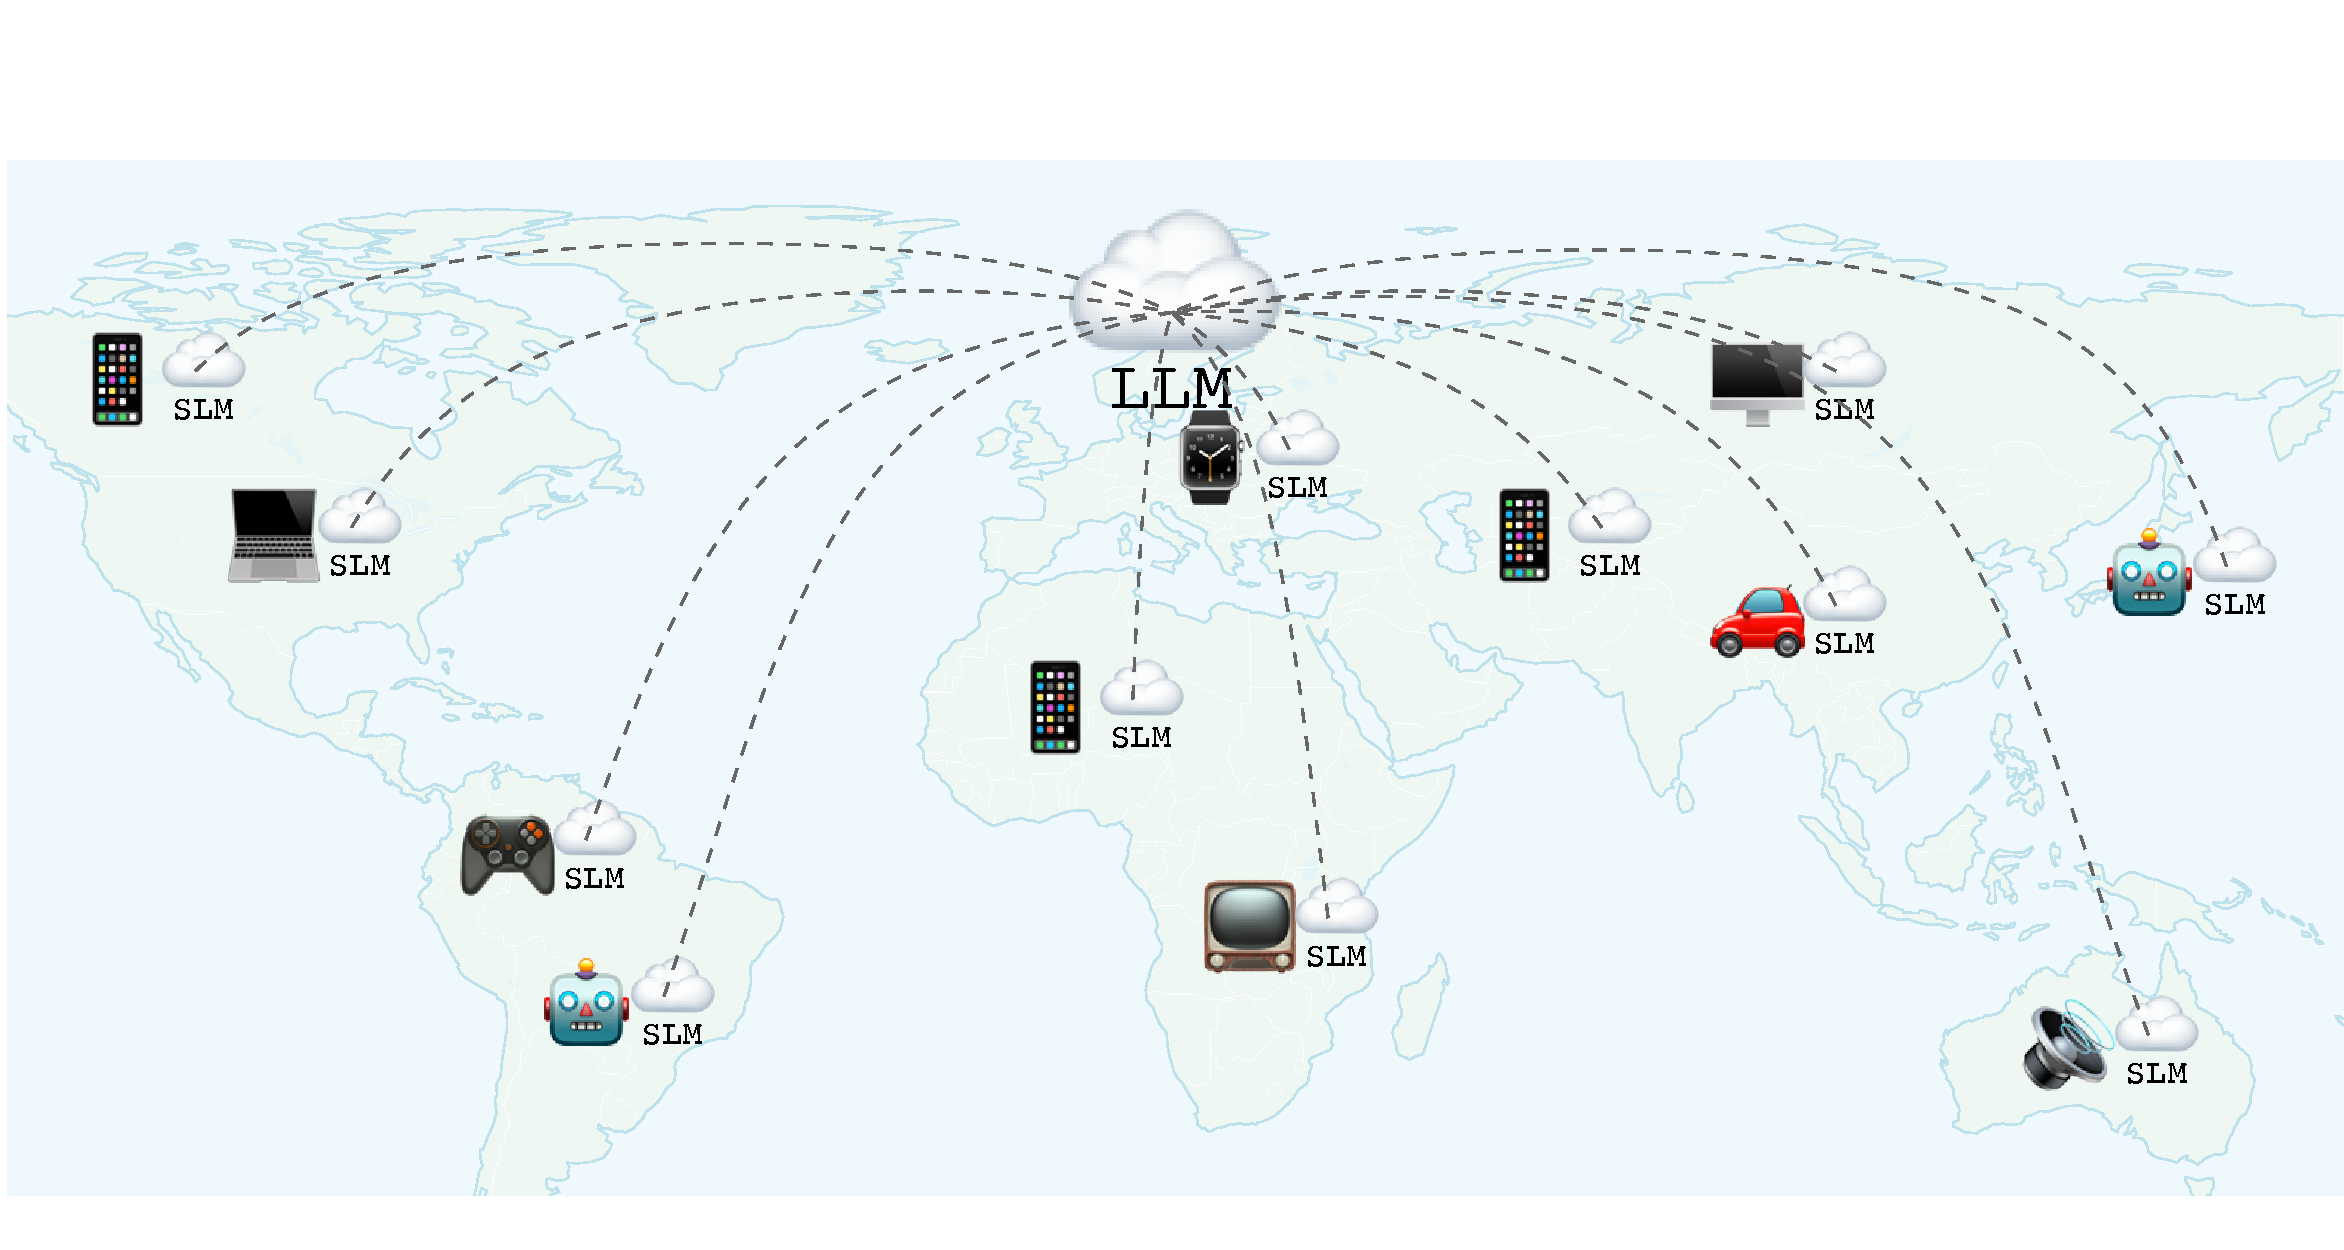
\includegraphics[width=0.8\linewidth]{./figs/fedllm.pdf}
    % \vspace{-20pt}
    \caption{Train Large Language Models with Small Edge Devices}
    \vspace{-15pt}
    \label{fig:fedllm}
\end{figure}
While some federated learning approaches allow training partial model parameters \cite{horvath2021fjord,alam2022fedrolex}, the enormous disparity between large language models and what edge devices can train—often orders of magnitude smaller due to inherently constrained resources—remains too vast to be effectively bridged by current FL frameworks.
Therefore, we need to develop a new federated learning paradigm that enables participants to collaboratively train a large language model even under extremely limited resources (as shown in Figure~\ref{fig:fedllm}).
\textbf{It is still an open problem to train large language models with small edge devices.} Therefore, we encourage the research community to develop novel distributed collaborative computing methods in two key directions:

\subsection{Heterogeneous Device Model Fusion: from Small to Large}\label{subsec:model_fusion}

The first direction addresses the fundamental challenge of model size disparity in federated learning. Modern large language models typically contain hundreds of billions of parameters, while edge devices have severely limited computational resources. This creates an enormous scale gap - the large target model may be hundreds or even thousands of times larger than what individual devices can handle. To bridge this gap, each edge device should run a small language model that matches its computational capacity. For example, while the central model may have 100 billion parameters, a resource-constrained mobile device might only handle a 100-million parameter model, representing a 1000x size difference. 
The key challenge then becomes how to effectively aggregate and fuse knowledge from these much smaller models into the large target model. 
We need novel techniques that can meaningfully combine insights from models operating at radically different scales while preserving the unique contributions of each small model. This requires fundamentally rethinking traditional model fusion approaches \citep{velasevic2023effects,azizan2019distributed} to handle such extreme parameter count disparities.

\subsection{Heterogeneous Device Compute Sharing: from Node to Cluster}\label{subsec:compute_sharing}

The second direction is to enable efficient compute resource sharing across heterogeneous devices by treating them as a unified compute cluster rather than independent nodes. Consider a smart home environment where multiple devices—smartphones, laptops, and desktop computers—could form a collaborative compute cluster. While each individual device has limited resources, their collective computing power could be substantial. For example, a laptop could handle intensive computational tasks, smartphones could manage coordination and lightweight processing, and desktop computers could contribute their onboard computing power. Meanwhile, other IoT devices such as smart speakers, security cameras, and vehicles could serve as data sources, providing valuable real-world inputs like voice commands, visual feeds, and environmental parameters. The language model would effectively run and train across this entire device cluster, leveraging both computing power and diverse training data from the environment.
This distributed execution requires new frameworks that can intelligently decompose and distribute model computations based on each device's capabilities and current load. The system must dynamically balance workloads - when the security cameras are idle at night, they could take on additional compute tasks, while during peak usage hours, the load could shift to other devices. 
This requires innovations in real-time resource allocation, task scheduling across heterogeneous hardware, and efficient inter-device communication protocols to ensure the collective computing power is optimally utilized \citep{zhao2024retrieval}.
